\documentclass[11pt]{article}
\usepackage[a4paper,margin=2cm]{geometry}
\usepackage{tikz}
\usetikzlibrary{positioning,calc}
\usepackage{booktabs}
\usepackage{array}
\usepackage{longtable}
\usepackage{tabularx}
\usepackage{parskip}
\pagestyle{plain}
\renewcommand{\arraystretch}{1.5}

\begin{document}

%% ================= PAGE 1: TREE =================
{\LARGE\bfseries CICIoT2023 labels}\\[4pt]
{\large 2-class, 8-class and 34-class: one tree}

\vspace{4pt}
Same rows every time, only the \emph{answer} the model must give changes.\\
Example row labelled \texttt{DDoS-SYN\_Flood}:\quad
binary $\rightarrow$ \textbf{Attack},\quad 8-class $\rightarrow$ \textbf{DDoS},\quad 34-class $\rightarrow$ \textbf{DDoS-SYN\_Flood}.

\vspace{6pt}
\begin{center}
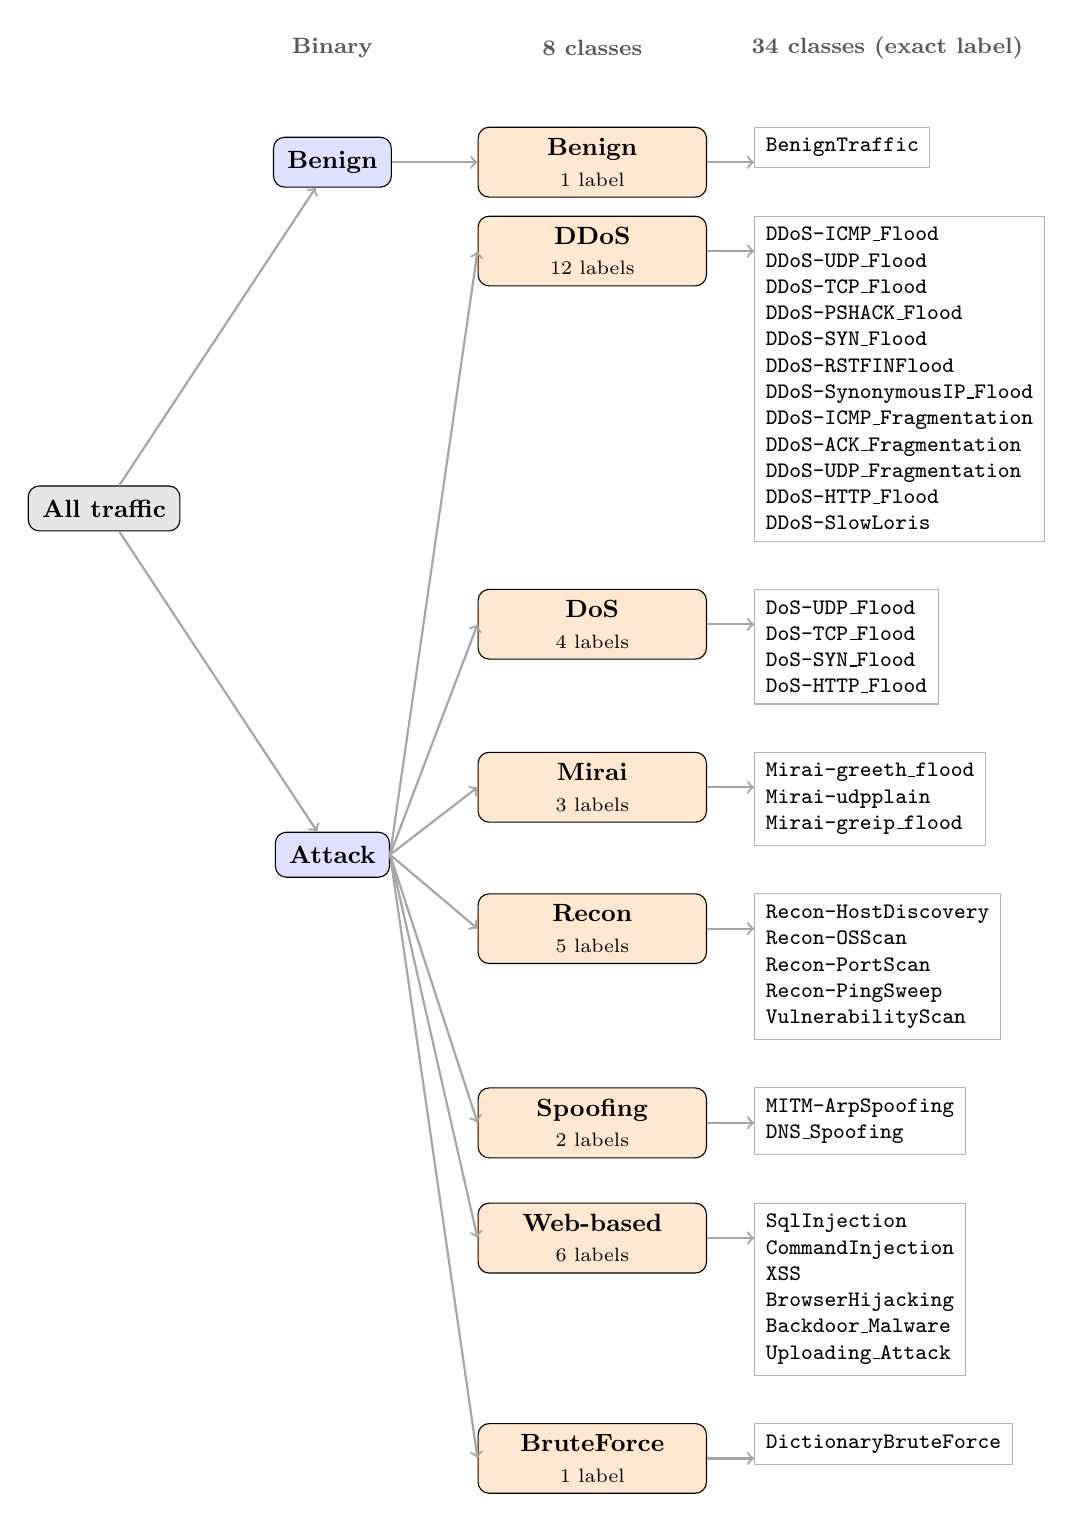
\begin{tikzpicture}[
  every node/.style={font=\small},
  lvl0/.style={draw, rounded corners, fill=gray!20, inner sep=5pt, font=\bfseries\small},
  lvl1/.style={draw, rounded corners, fill=blue!12, inner sep=5pt, align=center},
  fam/.style={draw, rounded corners, fill=orange!18, minimum width=2.9cm, inner sep=4pt, align=center},
  leaf/.style={draw=gray!60, align=left, inner sep=4pt, font=\footnotesize\ttfamily},
  edge/.style={->, gray!70, thick},
  hdr/.style={font=\bfseries\footnotesize, gray!70!black}
]
\coordinate (fcol) at (6.2,0);

% column headers
\node[hdr] at (2.9,1.0) {Binary};
\node[hdr] at (6.2,1.0) {8 classes};
\node[hdr, anchor=west] at (8.1,1.0) {34 classes (exact label)};

% families stacked vertically, each with its leaf box to the right
\node[fam, anchor=north] (Benign) at (fcol) {\textbf{Benign}\\{\scriptsize 1 label}};
\node[leaf, anchor=north west] (LBenign) at ([xshift=6mm]Benign.north east) {BenignTraffic};

\node[fam, anchor=north] (DDoS) at ([yshift=-6mm]LBenign.south -| fcol) {\textbf{DDoS}\\{\scriptsize 12 labels}};
\node[leaf, anchor=north west] (LDDoS) at ([xshift=6mm]DDoS.north east)
 {DDoS-ICMP\_Flood\\DDoS-UDP\_Flood\\DDoS-TCP\_Flood\\DDoS-PSHACK\_Flood\\DDoS-SYN\_Flood\\DDoS-RSTFINFlood\\DDoS-SynonymousIP\_Flood\\DDoS-ICMP\_Fragmentation\\DDoS-ACK\_Fragmentation\\DDoS-UDP\_Fragmentation\\DDoS-HTTP\_Flood\\DDoS-SlowLoris};

\node[fam, anchor=north] (DoS) at ([yshift=-6mm]LDDoS.south -| fcol) {\textbf{DoS}\\{\scriptsize 4 labels}};
\node[leaf, anchor=north west] (LDoS) at ([xshift=6mm]DoS.north east)
 {DoS-UDP\_Flood\\DoS-TCP\_Flood\\DoS-SYN\_Flood\\DoS-HTTP\_Flood};

\node[fam, anchor=north] (Mirai) at ([yshift=-6mm]LDoS.south -| fcol) {\textbf{Mirai}\\{\scriptsize 3 labels}};
\node[leaf, anchor=north west] (LMirai) at ([xshift=6mm]Mirai.north east)
 {Mirai-greeth\_flood\\Mirai-udpplain\\Mirai-greip\_flood};

\node[fam, anchor=north] (Recon) at ([yshift=-6mm]LMirai.south -| fcol) {\textbf{Recon}\\{\scriptsize 5 labels}};
\node[leaf, anchor=north west] (LRecon) at ([xshift=6mm]Recon.north east)
 {Recon-HostDiscovery\\Recon-OSScan\\Recon-PortScan\\Recon-PingSweep\\VulnerabilityScan};

\node[fam, anchor=north] (Spoofing) at ([yshift=-6mm]LRecon.south -| fcol) {\textbf{Spoofing}\\{\scriptsize 2 labels}};
\node[leaf, anchor=north west] (LSpoofing) at ([xshift=6mm]Spoofing.north east)
 {MITM-ArpSpoofing\\DNS\_Spoofing};

\node[fam, anchor=north] (Web) at ([yshift=-6mm]LSpoofing.south -| fcol) {\textbf{Web-based}\\{\scriptsize 6 labels}};
\node[leaf, anchor=north west] (LWeb) at ([xshift=6mm]Web.north east)
 {SqlInjection\\CommandInjection\\XSS\\BrowserHijacking\\Backdoor\_Malware\\Uploading\_Attack};

\node[fam, anchor=north] (Brute) at ([yshift=-6mm]LWeb.south -| fcol) {\textbf{BruteForce}\\{\scriptsize 1 label}};
\node[leaf, anchor=north west] (LBrute) at ([xshift=6mm]Brute.north east)
 {DictionaryBruteForce};

% binary level and root
\coordinate (bcol) at (2.9,0);
\coordinate (rcol) at (0,0);
\coordinate (attmid) at ($(DDoS.center)!0.5!(Brute.center)$);
\node[lvl1] (ben) at (Benign.center -| bcol) {\textbf{Benign}};
\node[lvl1] (att) at (attmid -| bcol) {\textbf{Attack}};
\coordinate (rootmid) at ($(ben.center)!0.5!(att.center)$);
\node[lvl0] (root) at (rootmid -| rcol) {All traffic};

\draw[edge] (root) -- (ben);
\draw[edge] (root) -- (att);
\draw[edge] (ben) -- (Benign);
\foreach \f in {DDoS,DoS,Mirai,Recon,Spoofing,Web,Brute}{\draw[edge] (att.east) -- (\f.west);}
\foreach \f in {Benign,DDoS,DoS,Mirai,Recon,Spoofing,Web,Brute}{\draw[edge] (\f.east) -- (L\f.west |- \f.east);}
\end{tikzpicture}
\end{center}

%% ================= HOW THE DATA WAS MADE =================
\newpage
\section*{How the data was captured}

\subsection*{The lab}
The Canadian Institute for Cybersecurity built a lab network with \textbf{105 real IoT devices} (cameras, smart plugs, speakers, sensors, hubs \dots).
Some extra machines (Raspberry Pis) were set up as \textbf{attackers}: they attacked the IoT devices while everything else kept running normally.
A switch copied (``mirrored'') \textbf{every packet on the network} to a capture computer, which saved them into \texttt{.pcap} files (Wireshark format).

\subsection*{Is this MQTT or CoAP data?}
\textbf{No, not specifically.} The capture is \emph{all} network traffic: TCP, UDP, ICMP, ARP, DNS, web, everything.
MQTT is just TCP traffic on port 1883 and CoAP is just UDP traffic on port 5683, so they are \emph{inside} the data as ordinary TCP/UDP packets.
There is no MQTT or CoAP column.

\subsection*{What is the ``window''? Is it 1 second?}
\textbf{No. The window is a number of packets, not a time.}
The authors computed the features for each packet, then \textbf{averaged them over a fixed number of consecutive packets}
Each row of the CSV is one such window. The paper (reference 1 of the TinyIDS PDF) gives the exact sizes:
\begin{itemize}
\item \textbf{100 packets} per row for all \textbf{DDoS, DoS and Mirai} attacks (floods produce huge amounts of packets).
\item \textbf{10 packets} per row for \textbf{Benign, Recon, Spoofing, Web-based and BruteForce}.
\end{itemize}

\textbf{Consequence:} the real time covered by a row changes a lot.
During a flood, 100 packets arrive in about a millisecond. In normal quiet traffic, 10 packets can take several seconds.
So you cannot say ``this row = 1 second of traffic''. This is the same problem you had with CICDDoS2019: if you want ``packets per second
towards a victim'', you have to compute it yourself on live traffic.

\subsection*{``Incoming'' and ``outgoing'': from where?}
Direction is seen from the \textbf{sender of the packets being measured}: outgoing = packets it sends, incoming = packets coming back to it.
In practice this did not work well in CICIoT2023. I checked your \texttt{test.csv}:
\begin{itemize}
\item \texttt{Srate} (outgoing rate) is \textbf{exactly equal} to \texttt{Rate} in all 1{,}176{,}851 rows.
\item \texttt{Drate} (incoming rate) is non-zero in only \textbf{74 rows} (0.006\%).
\end{itemize}
So \texttt{Srate} and \texttt{Drate} add nothing: \textbf{drop them and just use \texttt{Rate}}.

%% ================= FROM PACKETS TO ONE ROW =================
\newpage
\section*{From packets to one row: how a SYN flood is detected}

\subsection*{``If there is no time column, where does Rate come from?''}
Every captured packet carries a \textbf{timestamp}: the exact moment it arrived, to the microsecond (Wireshark shows it; in scapy it is \texttt{pkt.time}).
The authors \emph{had} these timestamps and used them to calculate \texttt{Rate}, \texttt{flow\_duration} and \texttt{IAT}.
Then they deleted the timestamp column from the CSV (the paper says it was only used for sorting).
So \textbf{time went into the calculation; only the results were kept.}

\subsection*{Worked example: one SYN-flood row (window = 100 packets)}
\begin{center}
\begin{tabular}{@{}c c c c@{}}
\toprule
Packet & Arrival time (s) & Flags & Size (bytes) \\
\midrule
1 & 12.000000 & SYN & 54 \\
2 & 12.000010 & SYN & 54 \\
3 & 12.000020 & SYN & 54 \\
\dots & \dots & \dots & \dots \\
100 & 12.001000 & SYN & 54 \\
\bottomrule
\end{tabular}
\end{center}

\begin{tabular}{@{}l l@{}}
\texttt{flow\_duration} & last time $-$ first time $= 12.001000 - 12.000000 = $ \textbf{0.001 s} \\
\texttt{Rate} & packets $\div$ duration $= 100 \div 0.001 = $ \textbf{100{,}000 packets/s} \\
\texttt{IAT} & average gap between packets $\approx$ \textbf{0.00001 s} \\
\texttt{syn\_flag\_number} & 100 SYN out of 100 $=$ \textbf{1.0} \\
\texttt{ack\_flag\_number} & 0 out of 100 $=$ \textbf{0.0} (nobody completes the handshake) \\
\texttt{TCP} & \textbf{1.0} \\
\texttt{Tot size} & \textbf{54 bytes}, all identical, so \texttt{Std} $\approx$ \textbf{0} \\
\end{tabular}

\vspace{6pt}
\textbf{Model sees:} huge rate + 100\% SYN + 0\% ACK + all TCP + tiny identical packets $\Rightarrow$ \textbf{SYN flood}.

\subsection*{Compare: normal web browsing (window = 10 packets)}
10 packets spread over about 2 seconds: \texttt{Rate} $\approx$ \textbf{5 packets/s}; a mix of SYN, ACK and PSH flags;
packet sizes from 54 to 1500 bytes, so \texttt{Std} is large. $\Rightarrow$ \textbf{Benign}.

And someone retrying a dead website (10 SYNs in 5 minutes): \texttt{Rate} $= 10 \div 300 \approx$ \textbf{0.03 packets/s}.
100\% SYN, but nowhere near flood speed $\Rightarrow$ does not look like the flood rows.

\subsection*{Doing the same thing live on the Raspberry Pi}
This is the ``Flow feature extractor'' box in the TinyIDS diagram: sniff packets, keep the last $N$, compute the same numbers, ask the model.

\begin{verbatim}
from scapy.all import sniff, TCP
N = 100          # 100 to match the flood rows in the dataset
buf = []

def on_packet(pkt):
    buf.append(pkt)
    if len(buf) == N:
        t = [float(p.time) for p in buf]
        duration = t[-1] - t[0]
        rate = N / duration if duration > 0 else 1e6
        syn  = sum(1 for p in buf if TCP in p and p[TCP].flags.S) / N
        ack  = sum(1 for p in buf if TCP in p and p[TCP].flags.A) / N
        tcp  = sum(1 for p in buf if TCP in p) / N
        size = sum(len(p) for p in buf) / N
        # ... same for the other features you keep ...
        # label = model.predict([[duration, rate, syn, ack, tcp, size, ...]])
        buf.clear()

sniff(iface="wlan0", prn=on_packet, store=False)
\end{verbatim}

\subsection*{Caveat: live numbers will not match the dataset exactly}
\begin{itemize}
\item The paper \textbf{does not publish the formulas} for most features and does not link its extraction code (see the next section).
My formulas above are the obvious, sensible ones, but the authors' versions may differ in details.
\item The dataset also mixes in flow information (e.g.\ \texttt{syn\_count} = SYNs ``in the same flow''), which a simple sliding window does not reproduce exactly.
\item Your testbed is different hardware and a different network from their lab.
\end{itemize}
\textbf{What to do about it:}
\begin{enumerate}
\item Train only on the \textbf{10--15 features you can compute yourself} (Rate, flow\_duration, IAT, flag fractions, protocol fractions, packet size stats). Drop Magnitue, Radius, Covariance, Variance, Weight, Srate, Drate.
\item Don't alert on a single window: alert when most windows in the last 1--2 seconds are flagged.
\item In the report, say that live testbed results are a \textbf{demonstration}, not the main accuracy figure. The TinyIDS PDF itself says this in its ``Validity note''.
\end{enumerate}

\newpage
\section*{What formulas do the authors actually use?}

\textbf{Short answer: mostly, they don't say.}

\vspace{4pt}
\fcolorbox{gray!60}{gray!6}{\begin{minipage}{0.96\textwidth}
\vspace{4pt}
The CICIoT2023 paper (Neto et al., \emph{Sensors} 2023, Table 4) gives:
\begin{itemize}
\item \textbf{Exact formulas for only 5 features:} \texttt{Magnitue}, \texttt{Radius}, \texttt{Covariance}, \texttt{Variance} and \texttt{Weight}. These are the ``incoming vs outgoing'' ones.
\item \textbf{Standard definitions} for the packet-size stats (\texttt{Tot sum}, \texttt{Min}, \texttt{Max}, \texttt{AVG}, \texttt{Std}) and the flag columns.
\item \textbf{Only one-line descriptions, no formula,} for \texttt{Rate}, \texttt{flow\_duration} and \texttt{IAT}.
For example, \texttt{Rate} is just described as ``rate of packet transmission in a flow''.
\item \textbf{Their tools:} \texttt{tcpdump} to split the captures, the Python library \texttt{dpkt} to read packets, and pandas/NumPy to average each window.
\item \textbf{The paper doesn't link any extraction code.} The only link it gives is to the dataset download page.
\end{itemize}
\textbf{Source:} \texttt{https://pmc.ncbi.nlm.nih.gov/articles/PMC10346235/}
\vspace{4pt}
\end{minipage}}

\vspace{10pt}
\textbf{Why this matters for you:} because the exact recipe for \texttt{Rate}, \texttt{flow\_duration} and \texttt{IAT} is not published,
nobody can reproduce those columns exactly. When you compute them live on the Pi you use the natural definitions
(packets $\div$ time, last time $-$ first time, average gap), and your numbers will be close but not identical to the dataset's.

\subsection*{Feature by feature}

\begin{longtable}{@{}>{\ttfamily\raggedright}p{3.6cm} >{\raggedright\arraybackslash}p{12.2cm}@{}}
\toprule
\textrm{\textbf{Feature}} & \textbf{What the paper gives} \\
\midrule
\endhead
Magnitue & \textbf{Formula:} $\sqrt{\mbox{avg incoming length} + \mbox{avg outgoing length}}$ \\
Radius & \textbf{Formula:} $\sqrt{\mbox{var incoming length} + \mbox{var outgoing length}}$ \\
Covariance & \textbf{Formula:} covariance of incoming and outgoing packet lengths \\
Variance & \textbf{Formula:} var(incoming lengths) $\div$ var(outgoing lengths) \\
Weight & \textbf{Formula:} \# incoming packets $\times$ \# outgoing packets \\
Tot sum, Min, Max, AVG, Std & Sum / min / max / mean / standard deviation of packet lengths in the flow (standard definitions). \\
Number & Number of packets in the flow. \\
flag numbers & Value (0/1) of that TCP flag in the packet, then averaged over the window. \\
flag counts & Number of packets with that flag in the same flow. \\
Rate, Srate, Drate & \textbf{Description only}, no formula: ``rate of packet transmission in a flow'' (all / outbound / inbound). \\
flow\_duration & \textbf{Description only}: ``duration of the packet's flow''. \\
IAT & \textbf{Description only}: ``time difference with the previous packet''. \\
Duration & Time-to-live (TTL) of the packet. \\
\bottomrule
\end{longtable}

\textbf{Bottom line:} only the five ``incoming vs outgoing'' features have exact formulas. For Rate, duration and IAT you must use the natural definitions, as in the example above.

%% ================= ATTACKS EXPLAINED =================
\newpage
\section*{The attacks explained}

\subsection*{First: DoS vs DDoS}
A \textbf{DoS} (Denial of Service) attack makes a device or service unusable by overloading it, usually by sending far more traffic than it can handle.
\begin{itemize}
\item \textbf{DoS} = the flood comes from \textbf{one} attacker machine.
\item \textbf{DDoS} (Distributed DoS) = the flood comes from \textbf{many} machines at once. Much harder to block because you cannot just ban one IP.
\end{itemize}
In the lab, DoS used one attacking Raspberry Pi and DDoS used many of them together. The flood \emph{types} are the same, which is why both families have SYN, UDP, TCP and HTTP floods.

\subsection*{Background you need: the TCP handshake}
Before two machines exchange data over TCP they do a 3-step handshake:
client sends \textbf{SYN} (``can we talk?'') $\rightarrow$ server replies \textbf{SYN-ACK} (``yes, I reserved space for you'') $\rightarrow$ client sends \textbf{ACK} (``great, let's go'').
Many floods abuse this.

\subsection*{DDoS family (12 labels) and DoS family (4 labels)}
\begin{description}
\item[SYN\_Flood] The attacker sends a huge number of SYN packets, usually with fake source IPs, and never sends the final ACK.
For each SYN, the server reserves memory and waits (a ``half-open'' connection). Its waiting list fills up, and real users can no longer connect.
Typical tool: \texttt{hping3 -S --flood}. \emph{This is the attack in your thesis.}
\item[SynonymousIP\_Flood] A SYN flood where the fake source IP is set to the \emph{victim's own IP}. The victim ends up trying to reply to itself, which confuses some network stacks and wastes more resources.
\item[TCP\_Flood] A flood of generic TCP packets (not just SYN) at high speed, to eat bandwidth and CPU.
\item[PSHACK\_Flood] Packets with the PSH and ACK flags set, pretending to be data in an already open connection. The server has to look each one up in its connection table before throwing it away. It also slips past defences that only watch for SYNs.
\item[RSTFINFlood] Packets with RST (``abort'') or FIN (``close'') flags. Again the server must check each against its connection table, costing CPU.
\item[UDP\_Flood] Massive numbers of UDP packets to random ports. UDP needs no handshake, so it is cheap to send. For each packet the victim checks whether any program listens on that port and often replies ``port unreachable'' (ICMP), wasting even more bandwidth.
\item[ICMP\_Flood] Also called a ping flood: nonstop ping (ICMP echo request) packets. The victim's link fills up and it spends CPU replying to each ping.
\item[ICMP / UDP / ACK\_Fragmentation] Big packets are split into small pieces (fragments) that the receiver must collect and reassemble. The attacker sends fragments that are broken or never complete. The victim keeps them in memory waiting for the missing pieces, and runs out of memory/CPU. The three labels differ only in which packet type is fragmented.
\item[HTTP\_Flood] Lots of normal-looking web requests (``GET /index.html'') sent to a web server. Each one makes the server do real work (read files, run code). Hard to filter because every single request looks legitimate.
\item[SlowLoris] A ``slow'' attack: the attacker opens many connections to a web server and sends the request headers \emph{very slowly}, a few bytes every few seconds, never finishing. The server keeps each connection open waiting, and soon all its connection slots are taken. Needs almost no bandwidth.
\end{description}
\textbf{DoS} labels (\texttt{DoS-UDP\_Flood}, \texttt{DoS-TCP\_Flood}, \texttt{DoS-SYN\_Flood}, \texttt{DoS-HTTP\_Flood}) are the same attacks as above, from a single machine.

\subsection*{Mirai family (3 labels)}
\textbf{What Mirai is.} Mirai is real malware from 2016. It scans the internet for IoT devices (cameras, routers, DVRs) that have Telnet open,
and tries to log in with a list of about 60 \textbf{factory-default passwords} like \texttt{admin/admin} or \texttt{root/12345}.
When it gets in, it infects the device, which becomes a \textbf{bot}. The bots wait for commands from the attacker's control server and then all flood a target together.
In October 2016 a Mirai botnet of hundreds of thousands of cameras and routers took down the DNS provider Dyn, which made Twitter, Netflix and Reddit unreachable for hours.
The source code was leaked, so many copies exist today. This is exactly why IoT security matters.

\begin{description}
\item[Mirai-greeth\_flood] Floods GRE packets. GRE is a ``tunnel'' protocol that wraps one packet inside another. Here each GRE packet carries a fake \textbf{Ethernet} frame, so the victim must unwrap every one.
\item[Mirai-greip\_flood] Same idea, but each GRE packet carries a fake \textbf{IP} packet.
\item[Mirai-udpplain] A plain UDP flood tuned for maximum packets per second (fewer random fields, so the bots can send faster).
\end{description}

\subsection*{Recon family (5 labels)}
\textbf{Recon} (reconnaissance) means scouting before an attack: what devices exist, what they run, and where the weak spots are. It does not damage anything by itself. Typical tool: \texttt{nmap}.
\begin{description}
\item[Recon-HostDiscovery] Find which IP addresses on the network are alive (e.g.\ \texttt{nmap -sn}).
\item[Recon-PingSweep] A simple form of host discovery: ping every address in a range and see who answers.
\item[Recon-PortScan] For one device, try many ports to see which are open. An open port answers SYN with SYN-ACK; a closed port answers with RST. That is why RST counts rise during scans. \emph{This is in your live demo.}
\item[Recon-OSScan] Send unusual probe packets and look at \emph{how} the device answers (TTL, TCP window size, option order). Each operating system answers slightly differently, which reveals whether it runs Linux, Windows, an embedded OS, etc.
\item[VulnerabilityScan] Automated tools (e.g.\ OpenVAS, Nessus) check each open service against a database of known security holes.
\end{description}

\subsection*{Spoofing family (2 labels)}
\begin{description}
\item[MITM-ArpSpoofing] On a local network, devices use ARP to ask ``who has IP 192.168.1.1 (the router)?''. The attacker keeps sending fake answers: ``that's me''. Victims then send their traffic to the attacker, who forwards it on, so nobody notices. The attacker sits in the middle (MITM = man-in-the-middle) and can read or change everything.
\item[DNS\_Spoofing] When a device asks DNS ``what is the IP of example.com?'', the attacker answers first with a fake IP. The device then connects to the attacker's server instead of the real one.
\end{description}

\subsection*{Web-based family (6 labels)}
These target web applications, e.g.\ a camera's or router's admin web page.
\begin{description}
\item[SqlInjection] The attacker types database code into a form field. Example: as the password, entering \texttt{' OR '1'='1}. If the site builds its database query by pasting in the input, the check becomes ``always true'' and the attacker logs in, or dumps the whole database.
\item[CommandInjection] Same idea, but the input is passed to the operating system's shell. Example: a ``ping this IP'' box where the attacker enters \texttt{8.8.8.8; cat /etc/passwd}, and the device runs both commands.
\item[XSS] Cross-site scripting: the attacker stores JavaScript inside a page (e.g.\ in a comment or device name). When someone else opens that page, the script runs in \emph{their} browser and can steal their login cookie.
\item[BrowserHijacking] Malicious code changes the victim's browser behaviour: redirects to other sites, changes the home page, injects ads, captures what they type.
\item[Backdoor\_Malware] Installing a hidden program on the device that lets the attacker come back later with remote access, bypassing the normal login.
\item[Uploading\_Attack] Abusing a file-upload feature (e.g.\ ``upload firmware'' or ``upload picture'') to upload a malicious script disguised as a normal file. If the server runs it, the attacker controls the server.
\end{description}

\subsection*{BruteForce family (1 label)}
\begin{description}
\item[DictionaryBruteForce] Try to log in again and again using a list of common passwords (a ``dictionary'' such as \texttt{rockyou.txt}) until one works. Usually against Telnet, SSH or a web login. The \textbf{MQTT brute force} in the TinyIDS demo is this same attack against the MQTT broker's username/password.
\end{description}

\subsection*{Benign}
\begin{description}
\item[BenignTraffic] Normal traffic from the 105 devices with no attack running: cameras streaming, plugs reporting status, hubs syncing, DNS lookups, updates, etc.
\end{description}

%% ================= PAGE: FAMILIES SUMMARY =================
\newpage
\section*{The 8 families: summary}

Row counts are from your \texttt{test.csv} (1{,}176{,}851 rows in total).

\begin{tabularx}{\textwidth}{@{}>{\bfseries}l X r@{}}
\toprule
Family & What it is & Rows in test \\
\midrule
DDoS & Flood a victim from \emph{many} machines at once: SYN, UDP, ICMP and HTTP floods, fragmented packets, and SlowLoris (keeps connections half-open so the server runs out of slots). & 855{,}981 (73\%) \\
DoS & The same kinds of floods, but from a \emph{single} machine. & 204{,}245 (17\%) \\
Mirai & Floods generated by the Mirai botnet, malware that infects cheap IoT devices (GRE and plain-UDP floods). & 66{,}749 (5.7\%) \\
Recon & Looking around before attacking: find live hosts, open ports, the operating system, known vulnerabilities. & 8{,}812 (0.7\%) \\
Spoofing & Pretending to be someone else: fake ARP replies (man-in-the-middle) or fake DNS answers. & 12{,}410 (1.1\%) \\
Web-based & Attacks on web apps: SQL injection, command injection, XSS, browser hijacking, uploading malware or backdoors. & 626 (0.05\%) \\
BruteForce & Guessing passwords from a word list. & 319 (0.03\%) \\
Benign & Normal traffic, no attack. & 27{,}709 (2.4\%) \\
\bottomrule
\end{tabularx}

\vspace{12pt}
\subsection*{Takeaways}
\begin{enumerate}
\item \textbf{Binary is easiest, 34-class is hardest.} For this project binary is enough; do 8-class if time allows.
\item \textbf{The data is very unbalanced.} DDoS and DoS are 90\% of all rows, while Web-based and BruteForce have only a few hundred. The model will be weak on the small ones; use class weights or undersample DDoS.
\item \textbf{Your live demo} (hping3 SYN/UDP flood, nmap port scan) falls under \textbf{DDoS/DoS} and \textbf{Recon}.
\end{enumerate}

%% ================= PAGE 3+: FEATURES =================
\newpage
\section*{The 46 features: what each column means}

\textbf{Key idea first.} Each row is \emph{averaged over a small window of consecutive packets}, it is not a single raw packet.
So a column that is 0 or 1 for one packet becomes a fraction:
\begin{itemize}
\item \texttt{syn\_flag\_number = 0.8} means \emph{80\% of the packets in that window had the SYN flag set}.
\item \texttt{TCP = 1.0} means \emph{every} packet in the window was TCP.
\end{itemize}

\vspace{6pt}
\begin{longtable}{@{}>{\ttfamily\raggedright}p{4.4cm} >{\raggedright\arraybackslash}p{11.4cm}@{}}
\toprule
\textrm{\textbf{Column}} & \textbf{Meaning (plain English)} \\
\midrule
\endfirsthead
\toprule
\textrm{\textbf{Column}} & \textbf{Meaning (plain English)} \\
\midrule
\endhead
\bottomrule
\endfoot

\multicolumn{2}{@{}l}{\large\bfseries A. Timing and speed}\\
flow\_duration & Time between the first and last packet of the flow. \\
Duration & \textbf{Misleading name:} it is actually the packet's \textbf{TTL} (time-to-live, i.e.\ how many router hops it has left). \\
Rate & Packets per second, measured over the window. \textbf{Very high during floods.} This is the only speed column worth using. \\
Srate & Meant to be the rate of \emph{outgoing} packets. \textbf{In your data it is identical to \texttt{Rate} in every row} $\Rightarrow$ useless, drop it. \\
Drate & Meant to be the rate of \emph{incoming} (reply) packets. \textbf{Non-zero in only 74 of 1.18 million rows} $\Rightarrow$ useless, drop it. (See ``How the data was captured''.) \\
IAT & Inter-arrival time: the gap since the previous packet. \\[6pt]

\multicolumn{2}{@{}l}{\large\bfseries B. TCP flags in the packet (fraction of window, 0 to 1)}\\
syn\_flag\_number & SYN = ``let's open a connection''. \textbf{High in SYN floods.} \\
ack\_flag\_number & ACK = ``got it''. Normal two-way traffic has lots of these. \\
fin\_flag\_number & FIN = ``I'm closing the connection politely''. \\
rst\_flag\_number & RST = ``abort this connection''. Closed ports reply with RST, so it rises during port scans. \\
psh\_flag\_number & PSH = ``deliver this data to the app right now''. \\
ece\_flag\_number, cwr\_flag\_number & Network congestion signals. Rare; usually 0. \\[6pt]

\multicolumn{2}{@{}l}{\large\bfseries C. Flag counters}\\
syn\_count, ack\_count, fin\_count, rst\_count, urg\_count & How many packets in the flow had that flag so far (a running count, not a fraction). \\[6pt]

\multicolumn{2}{@{}l}{\large\bfseries D. Packet header and protocol number}\\
Header\_Length & Size of the packet headers in bytes. \\
Protocol Type & IP protocol number: 6 = TCP, 17 = UDP, 1 = ICMP. Because it is averaged, it can be something like 6.4. \\[6pt]

\multicolumn{2}{@{}l}{\large\bfseries E. Which protocol is it? (fraction of window, 0 to 1)}\\
HTTP, HTTPS & Web traffic, plain and encrypted. \\
DNS & Name lookups (``what is the IP of google.com?''). \\
Telnet, SSH & Remote login: Telnet is unencrypted, SSH is encrypted. \\
SMTP & Sending e-mail. \\
IRC & Chat protocol, often used by botnets to receive commands. \\
TCP & Reliable, connection-based transport. \\
UDP & Fire-and-forget transport. \textbf{Equals 1 during UDP floods.} \\
ICMP & Ping and error messages. \textbf{Equals 1 during ping (ICMP) floods.} \\
ARP & ``Who has this IP address?'' on the local network. Abused in ARP spoofing. \\
DHCP & ``Please give me an IP address.'' \\
IPv & Is the packet IP at all. \\
LLC & Low-level link-layer frame. \\[6pt]

\multicolumn{2}{@{}l}{\large\bfseries F. Packet size statistics (bytes)}\\
Tot sum & Sum of the packet sizes. \\
Min, Max & Smallest and largest packet size. \\
AVG, Std & Average packet size and how much sizes vary. \\
Tot size & Average packet size. Floods use tiny, identical packets, so this is small and Std is near 0. \\
Number & Number of packets in the flow. \\[6pt]

\multicolumn{2}{@{}l}{\large\bfseries G. Incoming vs outgoing comparison}\\
Magnitue & $\sqrt{\mbox{avg incoming size} + \mbox{avg outgoing size}}$: overall ``how big'' the traffic is. (The typo is in the dataset itself.) \\
Radius & $\sqrt{\mbox{incoming variance} + \mbox{outgoing variance}}$: how much sizes vary in both directions. \\
Covariance & Do incoming and outgoing sizes move together (normal conversation) or not (one-way flood)? \\
Variance & Ratio of incoming-size variance to outgoing-size variance. \\
Weight & (number of incoming packets) $\times$ (number of outgoing packets). \\[6pt]

\multicolumn{2}{@{}l}{\large\bfseries H. The answer}\\
label & One of the 34 labels from the tree on page 1. This is what the model learns to predict. \\
\end{longtable}

\newpage
\section*{Why CICDDoS2019 looked so confusing}

That dataset was made with \textbf{CICFlowMeter}, where \emph{one row = one connection} between two machines.
Its column names use a few prefixes:

\begin{longtable}{@{}>{\bfseries\raggedright}p{3.6cm} >{\raggedright\arraybackslash}p{12.2cm}@{}}
\toprule
Prefix / word & Meaning \\
\midrule
\endhead
Fwd (forward) & Packets from the side that \emph{started} the connection (client $\rightarrow$ server). \\
Bwd (backward) & The \emph{replies} (server $\rightarrow$ client). \\
IAT & Inter-arrival time: the gap between packets. \\
Init\_Win\_bytes & TCP window size in the first packet. \\
Subflow & The connection cut into smaller pieces. \\
Bulk & Bursts of many packets sent back-to-back. \\
Active / Idle & How long the connection was busy vs quiet. \\
\bottomrule
\end{longtable}

Examples: \texttt{Total Fwd Packets} = how many packets the client sent;
\texttt{Bwd Packet Length Mean} = the average size of the server's replies.
In a SYN flood the server barely replies, so most \textbf{Bwd} columns are 0.

CICIoT2023 mostly drops the Fwd/Bwd split and uses ``incoming/outgoing'' instead (\texttt{Srate}, \texttt{Drate}, \texttt{Magnitue}, \texttt{Radius}, \dots).

\section*{Most useful columns for your demo attacks}

\begin{tabularx}{\textwidth}{@{}>{\bfseries}l X@{}}
\toprule
Attack & Columns that give it away \\
\midrule
SYN flood & \texttt{syn\_flag\_number}, \texttt{syn\_count}, \texttt{Rate}, \texttt{TCP} \\
UDP flood & \texttt{UDP}, \texttt{Rate}, \texttt{Tot size} \\
Port scan & \texttt{rst\_flag\_number}, \texttt{rst\_count}, \texttt{Number}, \texttt{Rate} \\
\bottomrule
\end{tabularx}

\end{document}
